\documentclass{InsightArticle}
\usepackage[dvips]{graphicx}

%%%%%%%%%%%%%%%%%%%%%%%%%%%%%%%%%%%%%%%%%%%%%%%%%%%%%%%%%%%%%%%%%%
%
%  hyperref should be the last package to be loaded.
%
%%%%%%%%%%%%%%%%%%%%%%%%%%%%%%%%%%%%%%%%%%%%%%%%%%%%%%%%%%%%%%%%%%
\usepackage[bookmarks,
bookmarksopen,
backref,
colorlinks,linkcolor={blue},citecolor={blue},urlcolor={blue},
]{hyperref}
\usepackage{subfigure}
\usepackage{amssymb,amsmath}

\usepackage{multirow}


%  This is a template for Papers to the Insight Journal. 
%  It is comparable to a technical report format.

% The title should be descriptive enough for people to be able to find
% the relevant document. 
\title{Primal/Dual Mesh with Application to Triangular/Simplex Mesh and Delaunay/Voronoi}

% 
% NOTE: This is the last number of the "handle" URL that 
% The Insight Journal assigns to your paper as part of the
% submission process. Please replace the number "1338" with
% the actual handle number that you get assigned.
%
\newcommand{\IJhandlerIDnumber}{1338} %TOMODIFY

% Increment the release number whenever significant changes are made.
% The author and/or editor can define 'significant' however they like.
\release{0.01}

% At minimum, give your name and an email address.  You can include a
% snail-mail address if you like.
\author{Humayun Irshad$^{1}$, St\'{e}phane Rigaud$^{1}$ and Alexandre Gouaillard$^{2}$}
\authoraddress{$^{1}$Image \& Pervasive Access Lab, National Centre for Scientific Research (CNRS), Fusionopolis, Singapore\\
$^{2}$Singapore Immunology Network, Agency for Science, Technology and Research (A*STAR), Biopolis, Singapore}
\begin{document}

%
% Add hyperlink to the web location and license of the paper.
% The argument of this command is the handler identifier given
% by the Insight Journal to this paper.
% 
\IJhandlefooter{\IJhandlerIDnumber}


\ifpdf
\else
   %
   % Commands for including Graphics when using latex
   % 
   \DeclareGraphicsExtensions{.eps,.jpg,.gif,.tiff,.bmp,.png}
   \DeclareGraphicsRule{.jpg}{eps}{.jpg.bb}{`convert #1 eps:-}
   \DeclareGraphicsRule{.gif}{eps}{.gif.bb}{`convert #1 eps:-}
   \DeclareGraphicsRule{.tiff}{eps}{.tiff.bb}{`convert #1 eps:-}
   \DeclareGraphicsRule{.bmp}{eps}{.bmp.bb}{`convert #1 eps:-}
   \DeclareGraphicsRule{.png}{eps}{.png.bb}{`convert #1 eps:-}
\fi


\maketitle


\ifhtml
\chapter*{Front Matter\label{front}}
\fi


% The abstract should be a paragraph or two long, and describe the
% scope of the document.
\begin{abstract}
\noindent
This document describes an implementation in ITK of an extension of ITK (QE) to handle primal and dual mesh in one container and a filter that allow to calculate primal/dual mesh from the primal mesh. This new data structure, \emph{itk::QuadEdgeMeshWithDual}, is an extension of the already existing \emph{itk::QuadEdgeMesh}~\cite{Gouaillard2006}, with all the same properties, with the dual mesh in additional. With the new data structure, we compute a primal/dual mesh from primal mesh that share common topology but different sampling. This paper is accompanied with the source code and examples that should provide enough details for users.
\end{abstract}
\IJhandlenote{\IJhandlerIDnumber}
\tableofcontents
%----------------- Section 1:Surfaces ----------------------------------
\section{Surfaces}
\subsection{Notion of deformable surfaces}

%---- Todo -- Remove deformable surfaces
%-----Todo -- add genus general formual and define components, border cells
A deformable surface can be characterized by vector of shape parameters $q = ( q_1, ... , q_{n_q})^T$ and vector of deformation parameters $q = ( d_1, ... , d_{n_d})^T$ that controls the application of a global transformation $T_d$ 
on the surface:
\begin{equation}
\begin{split}
	S(q,d)~=~T_d(S_q) ~:~\mathbb{R}^{n_q}~X~\mathbb{R}^{n_d}~X~\Omega~\longrightarrow~R^3 \\	
	(q_1,~... ,~q_{n_q},~d_1,~... ,~d_{n_d} )~\longmapsto~T_d(P_q(r,x))	\end{split}
\end{equation}
where (r,s) denotes a point of surface parameter domain $\Omega$.

A deformable surface can be represented by continuous and discrete models. With discrete representation, the geometry of surfaces is only known at a finite set of points. Continuous surfaces representation must be discretised for computational needs but they offer the ability to compute differential quantities such as surface norm or curvatures almost everywhere on the surface. Most discrete models are meshes defined as a set of points with some connecting relation that includes topological constraints. 
%-------------------------------------------------------------------
\subsection{Orientable 2-Manifold Mesh: A discrete real-world object}
The discrete surfaces of object are normally represented using mesh structure. The definition of surface mesh is of combinatorial nature~\cite{Kettner1999}, that improves reasoning about data structure like the same facet cannot appear on both sides of an edge. The surface mesh is a union of $C~=~V~\cup~E~\cup~F$ of three disjoint sets together with an incidence relation where V the vertices, E the edges and F the facets of the mesh. The incident relation on C must be symmetric. No two elements from the same set $V$, $E$, $F$ are incident. There are four additional conditions: (1) every edge is incident to two vertices, (2) every edge is incident to two facets, (3) for every incident pair of vertices or facets, there are exactly two edges incident to both and (4) every vertex and every facets is incident to at least one other element. The neighbourhood of a vertex are edges and facets which are incident to that vertex. Thus, the neighbourhood decomposes into disjoint cycles, where each cycle is an alternating sequence of edges and facets.

Genus is a topologically invariant property of a surface defined as the largest number of non-intersecting closed curves that can be drawn on the surface without separating it. Roughly speaking, it is the number of holes in a surface. Also, it is a complete invariant in the sense that, if two orientable closed surfaces have the same genus, then they must be topologically equivalent. The genus of a surface is related to the Euler characteristic $\chi$. For an orientable surface such as a sphere (genus 0) or torus (genus 1), the relationship is
\begin{equation}
\chi~=~2~-~2g
\end{equation}

There are two types of mesh representations i.e., manifold and non-manifold mesh as shown in figure~\ref{fig:meshes}. A mesh is manifold if (1) each edge is incident to only one or two facets and (2) the facets incident to a vertex form a close or an open fan i.e. for each point on a manifold surface there exists a neighbourhood that is homemorphic to the open disc. If every vertex has a closed fan, the given manifold has no boundary. If a vertex has a open fan, then edges that are incident to one facet; they are called border edges and they form the boundary of the manifold mesh. A non-manifold example would be two tetrahedra glued together at a single vertex or common edge as shown in figure~\ref{fig:meshes}. A mesh is a 2-manifold if and only if the neighbourhood of each vertex decomposes into a single cycle. The next distinction is between orientable and non-orientable mesh. A mesh is oriented if each cycle around a facet is oriented and if, for each edge, the two cycles of its two incident facets are oriented in opposite direction. A manifold mesh is orientable if there exists such an orientation. This new data structure only consider orientable 2-manifolds mesh representation with and without boundary. The set of discrete surfaces include triangulation and simplex meshes in order to extend the notion of discrete representation to include any surface representation as shown in figure~\ref{fig:triangulationSimplexMesh}.
\begin{figure}[!t]
	\centering
	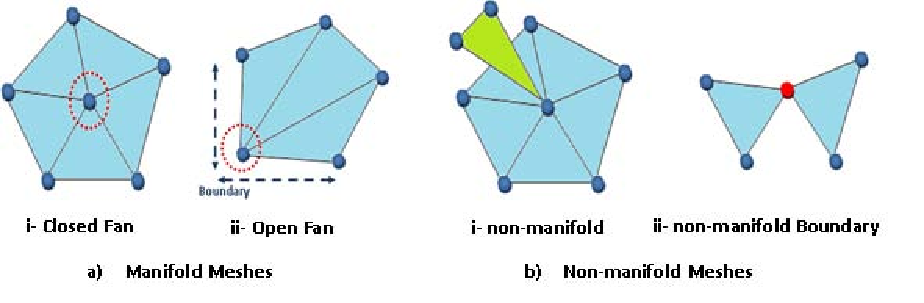
\includegraphics[width=155mm, height=40mm]{Meshes}
	\caption{Examples of Meshes}
	\label{fig:meshes}
\end{figure}
%------------------------------------------------------------------------
\subsection{Special Case A: Triangular Meshes}
A common representation of discrete surfaces are triangulation $\tau$ for which the surface $\mathbb{R} \subset S$ is composed of a set of adjacent triangles $T_i$, $i~=~1,~... ,~n$, such that 
\begin{itemize}
	\item $\cup_{i=1}^n~=~T_i~=~\mathbb{R}$.
	\item If $T_i~\cap~T_j~\neq~\phi$, then $T_i~\cap~T_j$ is either a common edge of $T_i$ and $T_j$ or a common vertex of $T_i$ and $T_j$. 
\end{itemize}
Given a triangular mesh $\tau$ of a regular region $R~\subset~S$ of a surface S, we shall denote by F the number of triangles(faces), by E the number of sides(edges), and by V the number of vertices of the triangulation. The number 
\begin{equation}
F~-~E~+~V~=~\chi
\end{equation}
is called the Euler-poincar$\acute{e}$ characteristic of the triangulation.
Each triangles of a triangulation shares at least one of its edge with a neighbouring triangle.
\begin{figure}[!t]
	\centering
	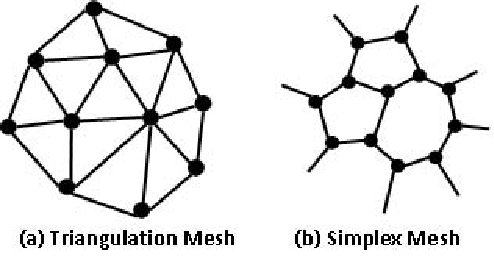
\includegraphics[width=100mm, height=40mm]{TriangulationSimplexMesh}
	\caption{Triangulation and Simplex Mesh}
	\label{fig:triangulationSimplexMesh}
\end{figure}
%----------------------------------------------------------------------
\subsection{Special Case B: Simplex Meshes}
Simplex meshes are used for discrete surface representation. Simplex meshes have two main properties, (1) each vertex is adjacent to a fixed number of neighbouring vertices: 2 for a contour (1-simplex mesh), 3 for a surface (2-simplex mesh) and 4 for tetrahedron (3-simplex mesh); and (2) the topology of a simplex mesh is dual of a triangulation. A $k$-simplex can be referred a $(k+1)$-connected mesh. For instance, a segment of non-zero length is a 1-simplex, a triangle (polygon) of non-zero area is a 2-simplex and a tetrahedron of non-zero volume is a 3-simplex mesh. Formally, a $k$-Simplex Mesh $(kSM)$ of $\mathbb{R}^3$ is defined as a pair $(V(M)$, $N(M))$ \cite{Delingette1994} where:
\begin{equation}
	V(M)~=~\{P_i\},~\{i~=~1,..., n\},~P_i\ ~\epsilon\  ~\mathbb{R}^3
	\label{eq1}
\end{equation}
\begin{equation}
	\begin{array}{c}
		N(M)~:~\{1,...,n\}~\longrightarrow~\{1,...,n\}^{k+1} \\
		i~\longmapsto~(N_1 (i), N_2 (i),...,N_{k+1} (i))
	\end{array}
	\label{eq2}
\end{equation}
\begin{equation}
	\begin{array}{c}
		\forall _i \ \epsilon \ \{1,...,n\},~\forall _j \ \epsilon \ \{1,...,k+1\},~\forall _l \ \epsilon \ \{1,...,k+1\}, \ l \neq j \\
		N_j (i)~\neq~i
	\end{array}
	\label{eq3}
\end{equation}
\begin{equation}
	N_l (i)~\neq~N_j (i)
	\label{eq4}
\end{equation}
$V(M)$ is the set of vertices of $M$ and $N(M)$ is the associated connectivity function. Equations ~(\ref{eq3}) and ~(\ref{eq4}) present a mesh from exhibiting loops. It is important to make a distinction between the topological nature of a mesh represented by its connectivity function N(M) and its geometric nature corresponding to the position of its vertices V(M). 

The structure of a simplex mesh is the one of a simply connected graph and does not in itself constitute a new surface representation. The simplex mesh representation has several desirable properties that makes them well suited for the recovery of geometric models from range data. The characteristics of simplex mesh for discrete surfaces includes generality (represents all types of orientable surfaces regardless of their genus and end numbers), simplicity (minimum number of vertices to represents a surface or shape) and adaptability.
%----------------- Section 2: Notion of Duality -------------------------
\section{Duality}
\subsection{Notion of Duality}
We define $A$ and $B$ to be dual meshes i.e., $B$ is dual of $A$ and vice versa, if the following conditions are satisfied.
\begin{itemize}
	\item The number of vertices of $A$ is the same as the number of face of $B$, so that they can be put into one-to-one correspondence.
	\item The number of vertices of $B$ is the same as the number of face of $A$, so that they can also be put into one-to-one correspondence.
	\item Each pair of vertices of $A$ that map to adjacent faces in $B$ is joined by an edge which can be put into correspondence with the common edge of the associated pair of faces of $B$. The edges that join adjacent vertices of $B$ can be put into the same correspondence with the common edges of the associated pairs of elements of $A$. 
\end{itemize}

Furthermore, we can say that $A$ and $B$ are orthogonal dual meshes, if, in addition to above conditions, when the meshes are superimposed, the two edges in every dual pair are orthogonal. Figure~\ref{fig:dualMeshes} illustrates the duality of meshes. Each boundary edge of a face in mesh $A$ is put into correspondence with a half-open edge in mesh $B$ which starts at the corner corresponding to that face in $A$ as shown in figure~\ref{fig:dualMeshes}.
\begin{figure}[!t]
	\centering
	\subfigure[2D Triangular Mesh with its Dual] {
		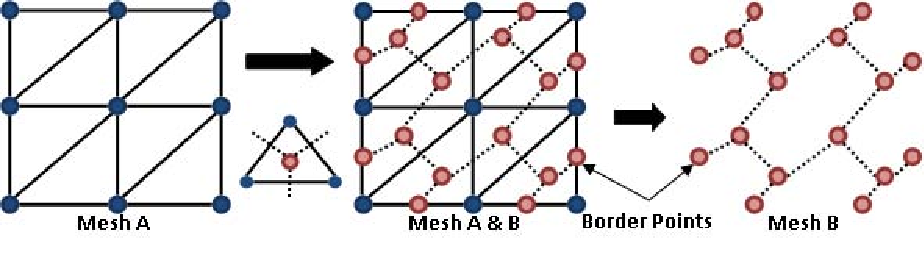
\includegraphics[width=160mm, height=40mm]{TriangleDualMesh}
		\label{fig:TriangleDualMesh}
		}
	\subfigure[2D Quad Mesh with its Dual] {
		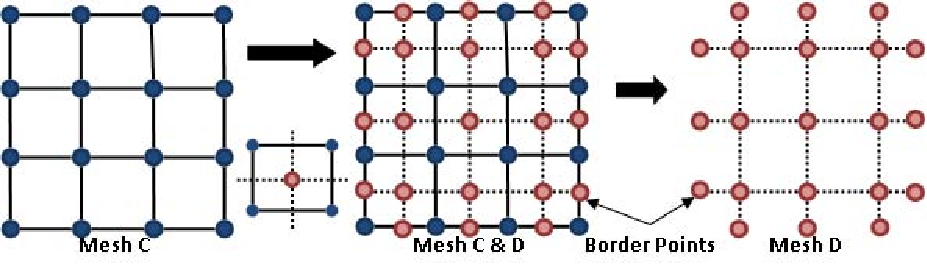
\includegraphics[width=160mm, height=40mm]{QuadDualMesh}
		\label{fig:QuadDualMesh}
		}
	\caption{Examples of Dual Meshes. (We also sampled the border points.)}
	\label{fig:dualMeshes}
\end{figure}
\subsection{Triangulation - Simplex Duality}
The most interesting way of considering simplex meshes is through duality of triangulations. The structure of a $k$-simplex mesh is indeed closely related to the structure of a $k$-triangulation. A $k$-triangulation of $\mathbb{R}^d$ is composed of $p$-simplices ( $1 \leq p \leq k$ ) which are the $p$-faces of the triangulation. We define a $p$-face of a $k$-simplex mesh as being the dual of a ($k-p$) simplices of a $k$-triangulation. For instance, a 1-face of a 2-simplex mesh is an edge and a 2-face of a 2-simplex mesh is polygon. In general, a $p$-face of a $k$-simplex mesh is a ($p-1$)-simplex mesh and is, therefore, made of $q$-faces ($q < p$). A Simplex mesh is said to be regular if all $p$-faces have the same number of vertices.

Simplex meshes are dual of triangulations. Thus, their connectivity functions N(M) are mapped by an homemorphism. Simplex meshes are topologically equivalent to triangulations but not geometrically equivalent. We can define a topological transformation that associates a $k$-simplex mesh to a $k$-triangulation. This transformation is pictured in figure~\ref{fig:simplexMeshes} and considers differently the vertices and edges located at the boundary of the triangulation from those located inside. 
\begin{figure}
	\centering
	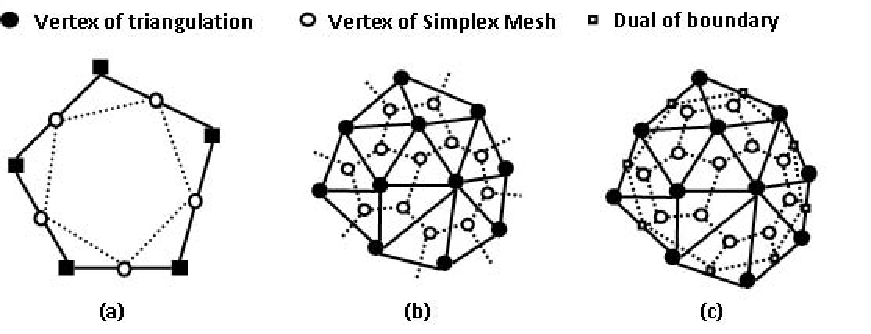
\includegraphics[width=150mm, height=50mm]{SimplexMesh_Examples}
	\caption{a) A 1-Simplex mesh and its dual; b) A 2-Simplex mesh and its dual triangulation; c) same as (b). The dual of the triangulation boundary is considered to extract the simplex mesh.}
	\label{fig:simplexMeshes}
\end{figure}
%------------------------------------------------------------------------
\subsection{Delaunay - Voronoi Duality}
Taking a set of point $\mathcal{P}$ in $\mathbb{R}^3$, the Delaunay triangulation of $\mathcal{P}$ is a specific triangulation of $\mathcal{P}$ that respects the Delaunay criterion stating that no point of $\mathcal{P}$ should be inside of the circumference circle of any triangle of the triangulation of $\mathcal{P}$. Taking a set of point $\mathcal{P}$ in $\mathbb{R}^3$, the Voronoi diagram (or tesselation) is the partition of $\mathbb{R}^3$  into $n$ polyhedral regions such as each region $T$ has a set of points in $\mathbb{R}^3$ which are closer to $T$ than to any other region.\\
The Voronoi diagram is the dual of the Delaunay triangulation, and the Delaunay triangulation is the dual structure of the Voronoi diagram. By dual, we mean to draw a line segment between two Voronoi vertices if their Voronoi polygons have a common edge, or in more mathematical terminology: there is a natural bijection between the two which reverses the face inclusions. The duality between Delaunay triangulations and Voronoi diagram is geometric because it depends on the position of its vertices.
%----------------- Section 3: Implement Duality in iTK--------------------
\section{Implement Duality in ITK}
%-------------------------------------------------------------------------
\subsection{Existing Data Structure for Meshes in ITK}
The \emph{QuadEdgeMesh} data structure in itk, as depicted in figure~\ref{fig:QuadEdgeMeshStructure}, can handle discrete 2-manifold surfaces. It actually store the geometry and both primal and dual topology. It has a constant complexity local accesses an modifications. The \emph{QuadEdgeMesh} data structure is a 3 layers structure in which the bottom layer is called QuadEdge (\emph{QE}) layer that represents the topology, the intermediate layer is called QE Geometric (\emph{QEGeom}) layer that linking topology and geometry and finally the upper layer is native to ITK called ITK layer. The \emph{QE} data structure is presented in detail in~\cite{Gouaillard2006}. For each edge, there are 4 \emph{QE}s in the structure as illustrated in figure~\ref{fig:QuadEdge}. It contains two primal \emph{QE}s and two dual \emph{QE}s. For the sake of simplicity, we only draw connection for one point and one face from \emph{QE} to \emph{QEGeom} and \emph{QEGeom} to ITK layer as shown in figure~\ref{fig:QuadEdge}, conversely both points and faces are equally linked in the data structure. This data structure only need three operators as \emph{Rot}, \emph{Onext} and \emph{Splice} to implement all other modifications (Euler operator) and accessibility of the mesh. 
\begin{figure}
	\centering
	\subfigure[QuadEdgeMesh structure] {
		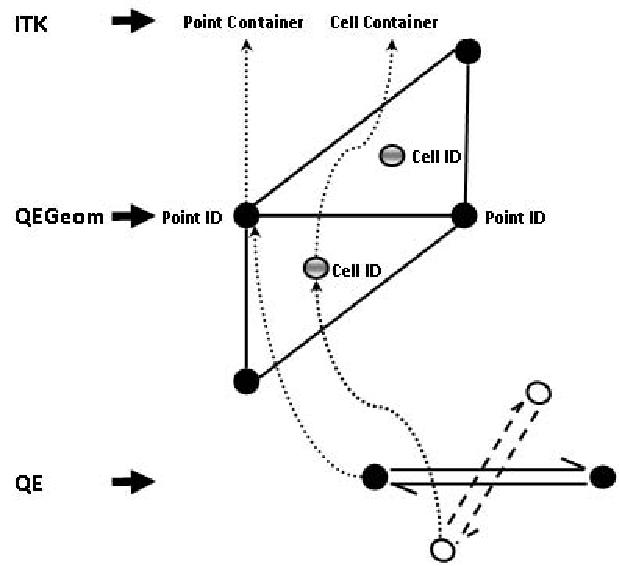
\includegraphics[width=100mm, height=70mm]{QuadEdgeMesh_Structure}
		\label{fig:QuadEdgeMesh}
		}
	\subfigure[QuadEdge structure] {
		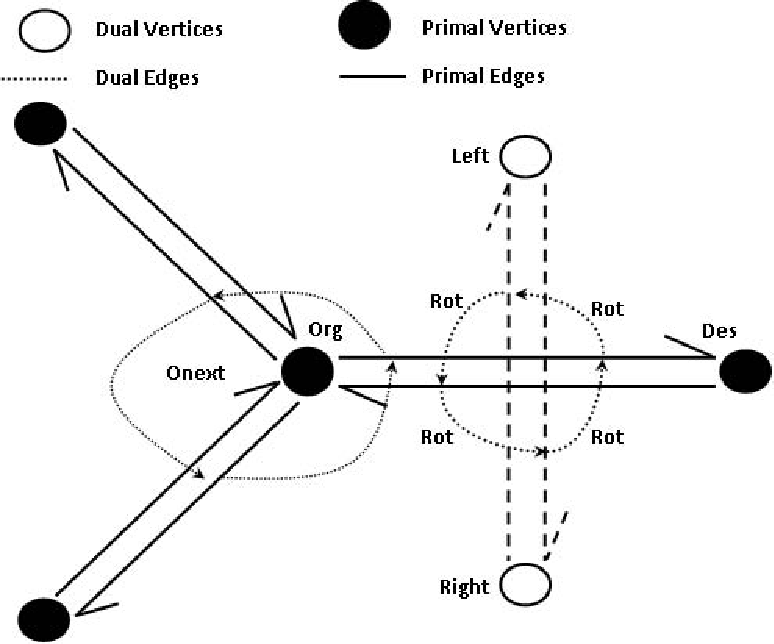
\includegraphics[width=60mm, height=50mm]{QuadEdgeMesh}
		\label{fig:QuadEdge}
		}
	\caption{Existing data structures}
	\label{fig:QuadEdgeMeshStructure}
\end{figure}
Currently, \emph{QuadEdgeMesh} data structure have topological duality but lack geometrical duality as represent in table~\ref{table:existingStructure}. There are only few filters available in ITK that transform triangular mesh to simplex mesh but it is specific not generic to duality. Additionally, in many cases it is of much interest to have the both representation of a discrete surface directly integrated in the structure. Our contribution includes an extension of data structure that contain both primal and dual mesh simultaneously, a filter that transform primal mesh to primal/dual mesh just using single data structure and an adaptor for displaying dual mesh.
\begin{table}
	\begin{center}
		\caption{QuadEdgeMesh Data Structure}
		\label{table:existingStructure}
		\begin{tabular}{ p{3cm} p{3cm} p{3cm} }
			\hline	
			\noalign{\smallskip} 
			{\bf  }	& {\bf Primal} & {\bf Dual} \\
			\noalign{\smallskip}	
			\hline  	
			\noalign{\smallskip}
			Geometry & Yes & \textbf{\underline{No}} \\ 
			Topology & Yes & Yes \\ 
			\hline
	\end{tabular}
	\end{center}
\end{table}
%--------------------------------------------------------------------
\subsection{Extension in data structure, \emph{QuadEdgeMeshWithDual} data structure}
We create a new class \emph{itk::QuadEdgeMeshWithDual} derived from \emph{itk::QuadEdgeMesh}. This class now stores both primal and dual mesh simultaneously. The new design of \emph{QuadEdgeMeshWithDual} data structure is contained double reference i.e., one for primal point to dual cell and one for primal cell to dual point as depicted in figure~\ref{fig:QuadEdgeMeshWithDual}. For the sake of simplicity, we only draw connection from QE layer to QEGeom layer and QEGeom layer to ITK layer for one point and one face instead of both points and both faces as shown in figure~\ref{fig:QuadEdgeMeshWithDual}. The primal and dual overlapping structures of connections at QEGeom layer is shown in figure~\ref{fig:QEGeomLayer}.
\begin{figure}
	\centering
	\subfigure[QuadEdgeMeshWithDual's layers] {
		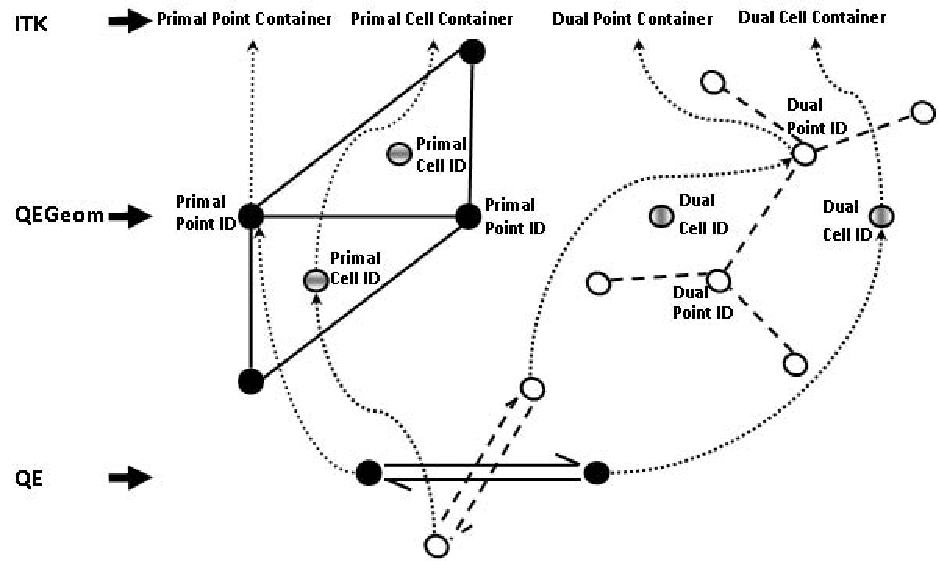
\includegraphics[width=100mm, height=70mm]{QuadEdgeMeshWithDual_Structure}
		\label{fig:QuadEdgeMeshWithDual}
		}
	\subfigure[QEGeom Layer of QuadEdgeMeshWithDual] {
		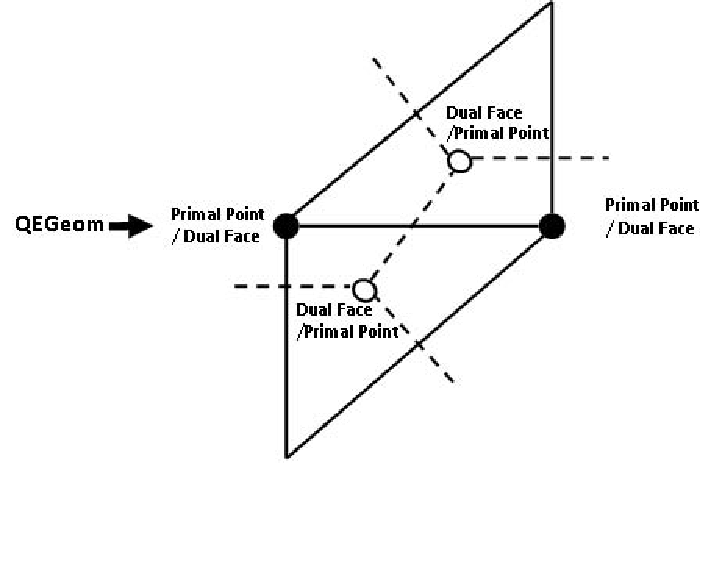
\includegraphics[width=60mm, height=62mm]{QEGeomLayer}
		\label{fig:QEGeomLayer}
		}
	\caption{QuadEdgeMeshWithDual data structure}
	\label{fig:QuadEdgeMeshWithDualFull}
\end{figure}
Furthermore, this class contains three new containers; \emph{DualPointsContainer} for dual points, \emph{DualCellsContainer} for dual cells and \emph{DualEdgeCellsContainer} for boundary edges and three new functions; \emph{AddDualPoint} for adding dual point, \emph{AddDualFace} for dual cells (polygon) and \emph{AddDualEdge} for boundary edges. 

In order to keep the primal-dual references in a single data structure, we have two design options. In first design, we use to maintain two look up tables; one table for storing references of primal cell to dual point and and second table for primal point to dual cell. The advantage of this approach is backward compatibility of code and test cases. The bad side of this design is to maintain these tables that having the complexity $nlog(n)$ causing severe degradation of performance in case of large mesh. In second design, we modify the existing data structure by adding two reference pair; primal point to dual cell and primal cell to dual point as shown below. With this design, no look up table is required to maintain the primal and dual references. So it is very efficient approach but not compatible with respect to previous code and test cases. 

%--- Todo -- illustrate both old and new code for origin ref type
\begin{verbatim}
typedef GeometricalQuadEdge< std::pair<PointIdentifier, CellIdentifier>,
                             std::pair<CellIdentifier,  PointIdentifier>,
                             PrimalDataType, 
                             DualDataType
                             > QEPrimal;
\end{verbatim}
A summaries of changes in new data structure can be depicted in Table~\ref{table:secondDesign}
\begin{table}
	\begin{center}
		\caption{Summaries of changes in new data structure}
		\label{table:secondDesign}
		\begin{tabular}{ l|l|c|c }
			\hline	
			{\bf  }	& {\bf } 	& {\bf Old Data Structure}	& {\bf New Data Structure}\\
			\hline  	
			\multirow{2}{*}{\vspace{0.5cm}Changes}  & OriginRef Type & Point ID & $Pair<Point, Cell>$ \\
			  &  &  Cell ID & $Pair<Cell, Point>$ \\ 
			Additions & Dual Containers & \multirow{3}{*}{-} & \emph{DualPointsContainer} \\ 
			  &  &  & \emph{DualCellsContainer} \\ 
			  &  &  & \emph{DualEdgeCellsContainer}\\
			Not yet implemented & Dual Data Containers &  - &  -  \\
			\hline
	\end{tabular}
	\end{center}
\end{table}
%----------------------------------------------------------------------
\subsection{Primal to primal/dual filter }
In order to transform primal mesh into dual mesh, we also create a new filter called \emph{itk::QuadEdgeMeshToQuadEdgeMeshWithDualFilter}. This filter is templated with \emph{QuadEdgeMeshWithDual} data structure. This filter generate dual mesh from primal mesh in three phases; first phase is computing dual point from primal cells, second phase is computing dual cells from primal points, and in last phase, primal borders edges are used to generate dual border cell.

We also implement a new adaptor for showing dual mesh.
%-----------------------------------------------------------------------
\subsubsection{Dual point functor}
As explained before, there is no geometrical duality between the primal and the dual. Therefore any formula that compute points that satisfy the criteria of duality detailed in section 2.1 can be use. In order not to have a single option that may limits the application of the filter, a functor is used to compute the dual point. Depending on the case faced, the user is able to choose from the already two existing dual point functor, or use his own functor. Except from the classic ITK macro, \emph{typedef} definition and constructor/destructor, the functor has only one method where the process is done.
\begin{verbatim}
template< class TInputMesh, class TOutputMesh=TInputMesh>
class DualPointFunctor
{
typedef typename TInputMesh::CellsContainer    CellsContainer;
typedef typename CellsContainer::ConstIterator CellIterator;
...
inline OutputPointType 
operator() ( const TInputMesh* primalMesh, CellIterator cellIterator ) 
  {...}
};
\end{verbatim}
\paragraph{\textbf{Barycentre}}
In general cases, the barycentre of each face of the mesh is used for the dual point. It has the advantage to be costless to calculate, to always be located inside its corresponding face and to work with any type of mesh. The following equation is used to compute the centre
\begin{equation}
\label{eq5}
M~=~\frac{P_1~+~P_2~+~\mathnormal{...}~+~P_n}{n}
\end{equation}
where $P_1,~P_2, ...,~P_n$ are the points retrieve from the current cell.

\paragraph{\textbf{Circumcentre}}
The circumcentre is a particular dual point of triangle mesh. It is the centre of the circumference circle of a triangle and is determine by the crossing point of the perpendicular bisectors, is not always include in its primal cell face, and more costly to compute. The interest of this dual point is in the case of the Delaunay triangulation in order to obtain its dual, the corresponding Voronoi tesselation. The following equation is used to compute the centre
\begin{equation}
\label{eq6}
M~=~P_1~+~\frac{|P_3-P_1|^2~[(P_2-P_1)\times(P_3-P_1)]\times(P_2-P_1)~+~|P_2-P_1|^2~[(P_3-P_1)\times(P_2-P_1)]\times(P_3-P_1)}{2~|(P_2-P_1)\times(P_3-P_1)|^2}
\end{equation}
where $P_1,~P_2,~P_3$ are the points retrieved from the current triangle, and $\times$ the cross product. In order to simplify the calculus and avoid the use of square roots the edge length are squared and the coordinates of all the point relative to the first point $P_1$ are used. Due to the floating-point errors such solution may be unstable in the case of the denominator is close to $0$. To prevent such case, the exact geometric predicate implemented for ITK \cite{Moreau2011} is use for the cross product calculation.
%-----------------------------------------------------------------------
\subsubsection{Dual borders calculation}
As shown in figure \ref{fig:dualMeshes}, the dual of a primal mesh that contain a border is not a closed mesh. The dual edge point obtain from the primal border are not included into any faces of the dual. This representation may be problematic to some other process which may not take into account the \emph{EdgeContainer} that store the edges in the \emph{QuadEdgeMesh} structure, and therefore discard edges that are not part of any face (\emph{e.i.} Mesh writting filter). If the dual edge point are not compute, the effect still occur but is less important that in the previous case. Another option is to create a border by connecting the dual edge point, however this solution may lead to some visual errors, such as overlapping faces in the dual, in particular configuration. The \emph{SetBorders()} methods allow the user to decide how the filter should manage the borders (Fig. \ref{fig:BorderManagment}). By default the filter will compute the dual edge point and create a border to the dual mesh.
\begin{figure}
	\centering
	\subfigure[Dual without dual edge point] {
		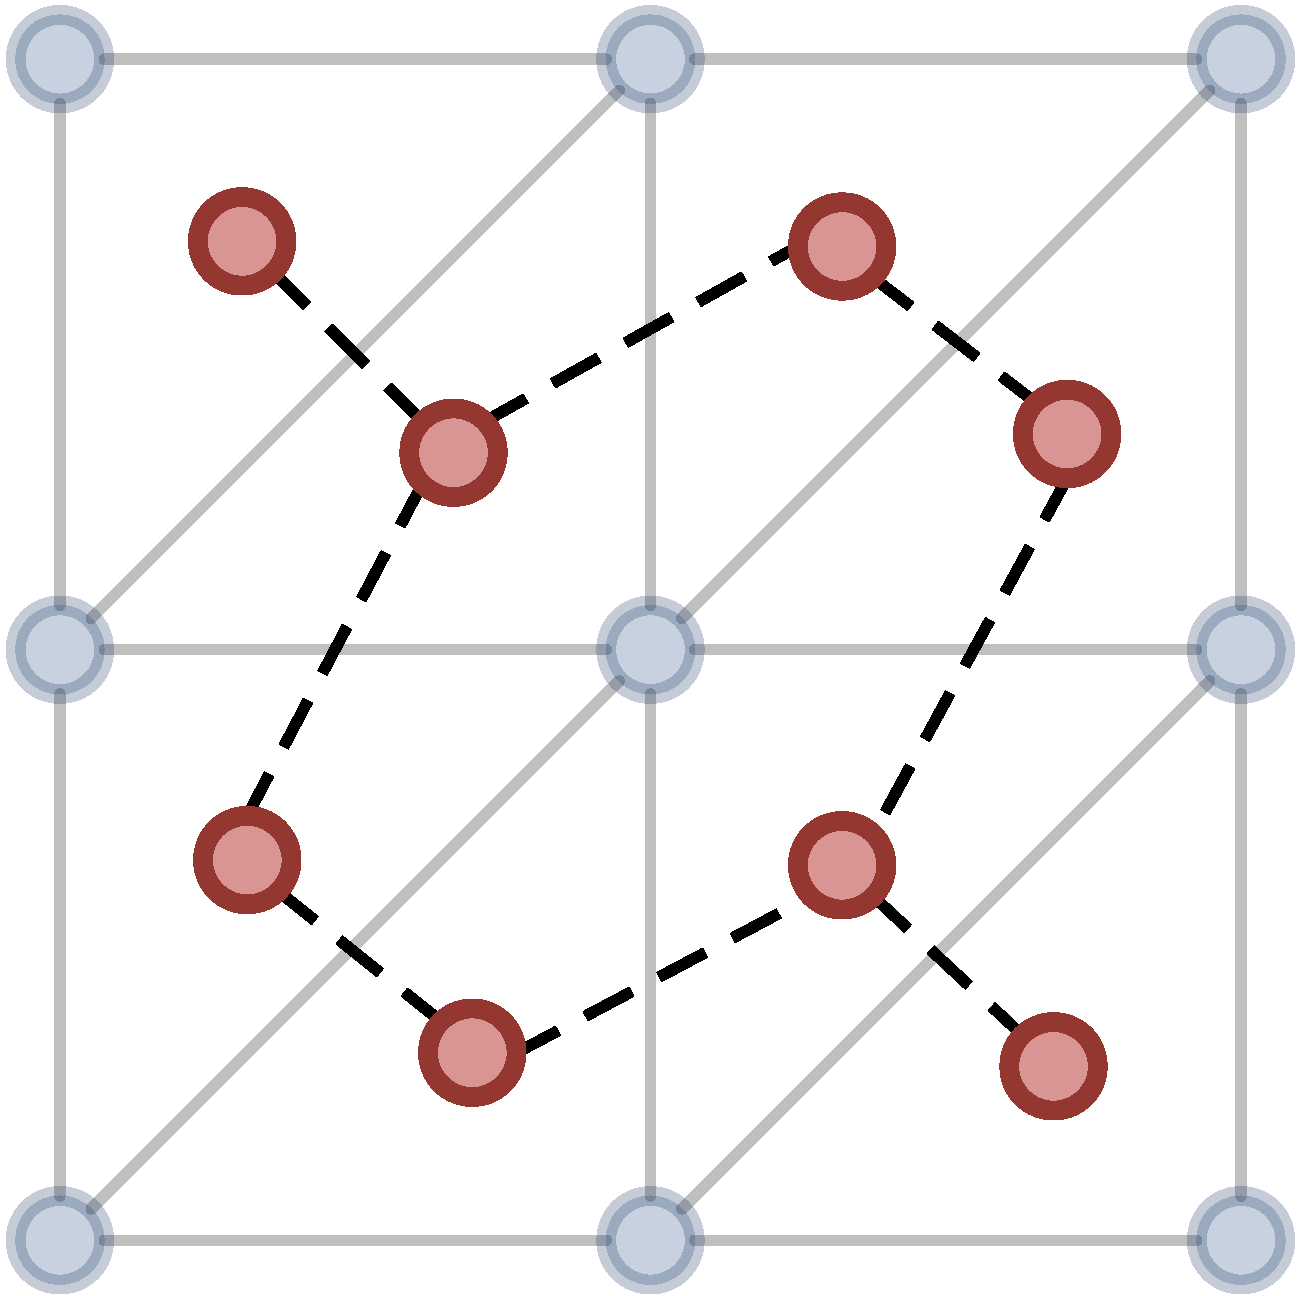
\includegraphics[width=0.3\textwidth]{border1}
		\label{fig:BorderManagment1}
		}
	\subfigure[Dual with dual edge point] {
		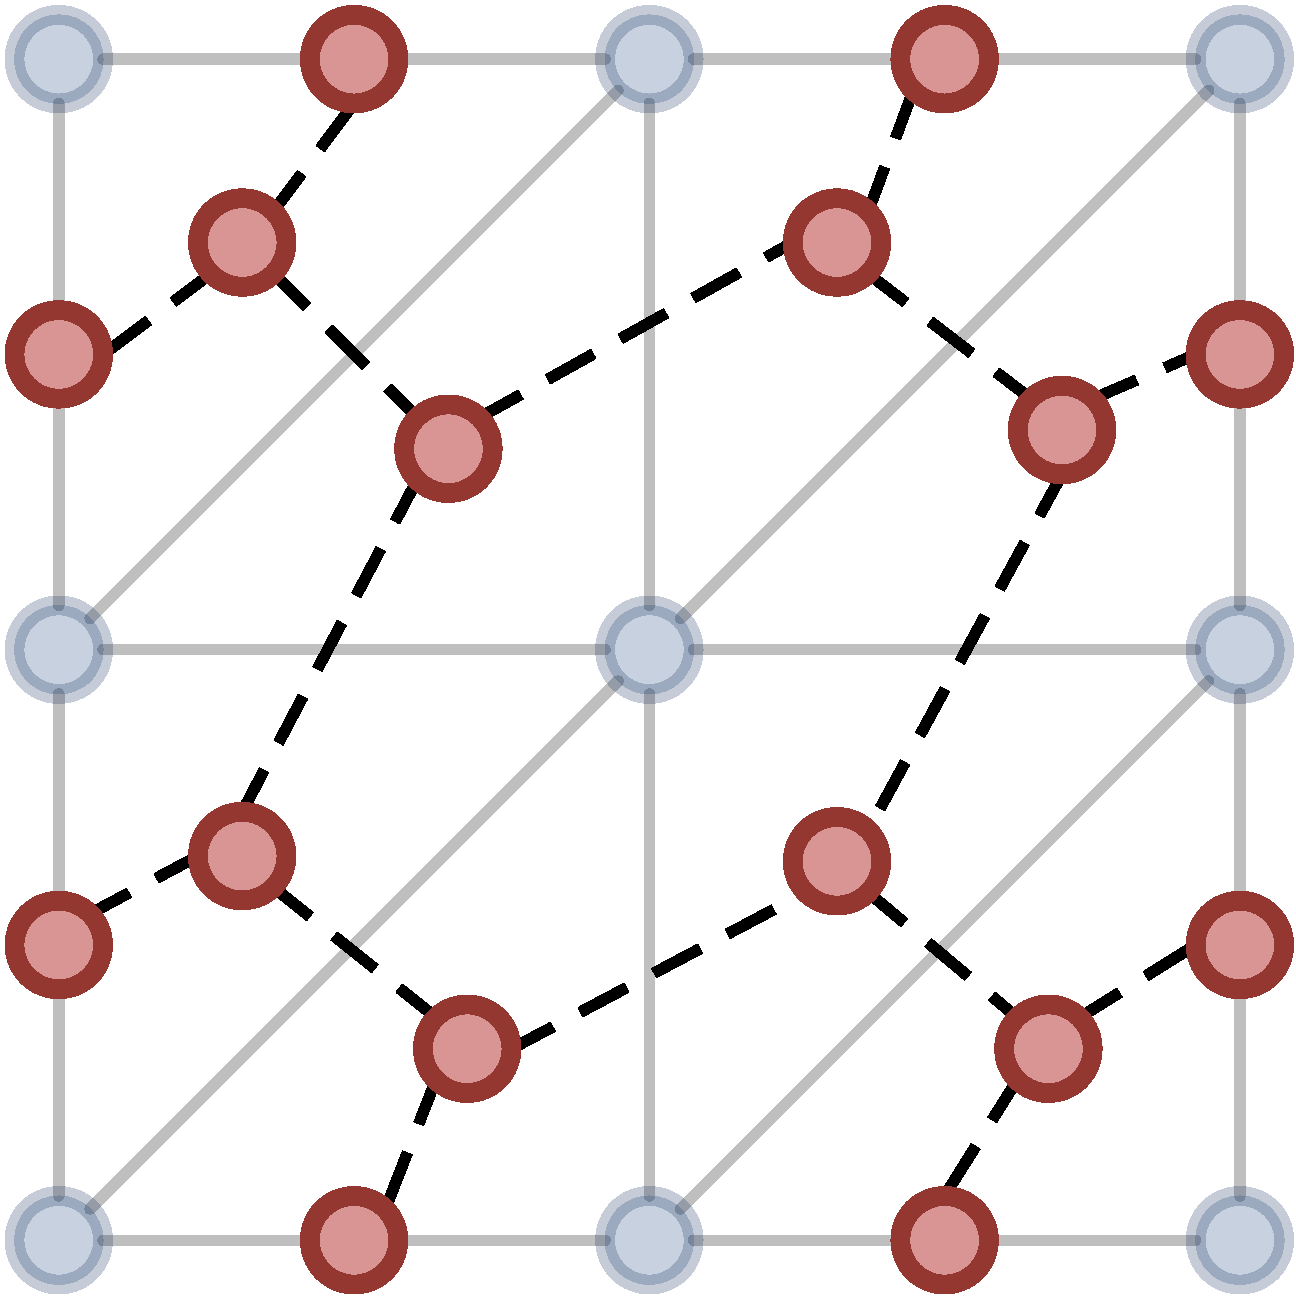
\includegraphics[width=0.3\textwidth]{border2}
		\label{fig:BorderManagment2}
		}
	\subfigure[Dual with dual edge point border] {
			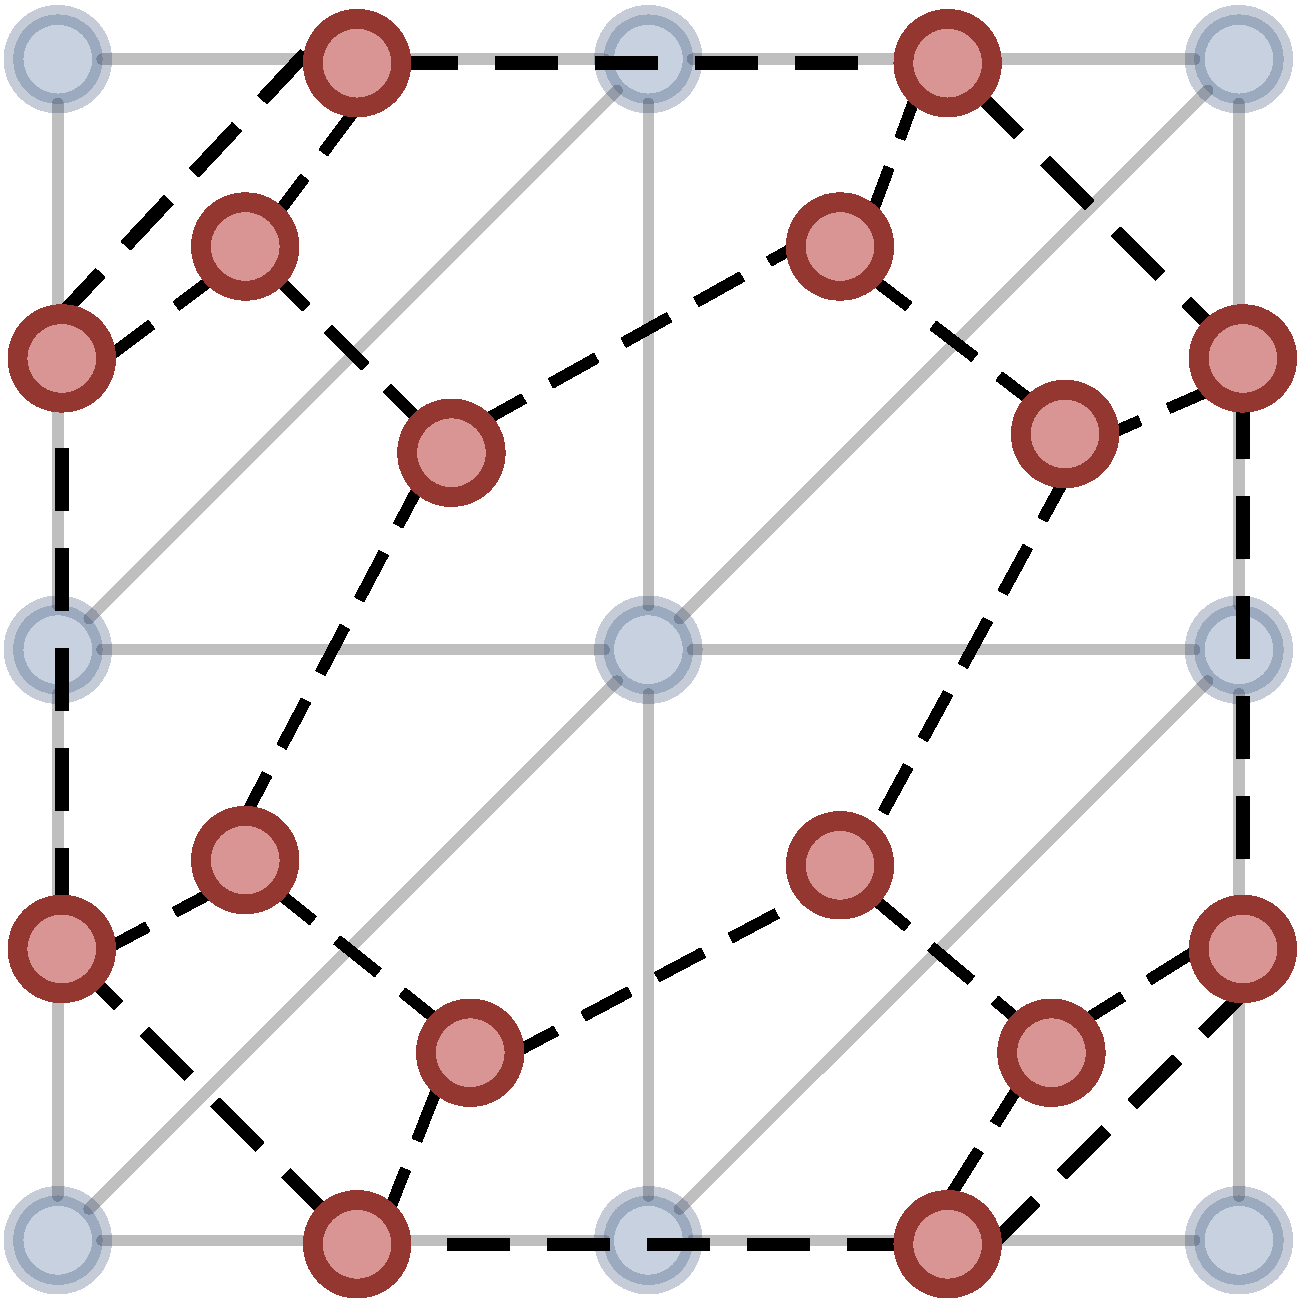
\includegraphics[width=0.3\textwidth]{border3}
			\label{fig:BorderManagment3}
			}
	\caption{Dual borders management options}
	\label{fig:BorderManagment}
\end{figure}

%-----------------------------------------------------------------------
\section{Validation}
%-----------------------------------------------------------------------
\subsection{Test on planer triangular to simplex mesh with and without holes}
We create a square triangulated (primal) mesh as shown in figure~\ref{fig:subfiga}. Green color represents primal points and cells. From this primal mesh, we would try to generate dual mesh. First, we generate dual points using the \emph{BarycentreDualPointFunctor} on the primal cells as shown in figure~\ref{fig:subfigc} with red points. We add these dual points in \emph{m\_DualPointsContainer} of itk::QuadEdgeMeshWithDual by using \emph{AddDualPoint()}. Second, we iterate around each primal point to form dual cells and add dual cell in \emph{m\_DualCellsContainer} of \emph{itk::QuadEdgeMeshWithDual} by using \emph{AddDualFace()}. By doing this we generate all dual cells except boundary cells. Dual cell are represented by red color in figure~\ref{fig:subfigc}.\\
In order to tackle borders, first we get boundary edges of primal mesh. Select one boundary edge from list; create a new point (dual) in the middle of edge and add in \emph{m\_DualPointsContainer} of \emph{itk::QuadEdgeMeshWithDual} by using \emph{AddDualPoint(...)}.  
In figure~\ref{fig:subfige}, red points on border lines represent boundary points of dual mesh. Then, find the dual point associated with the face on the left and make an edge between these two dual points. Now iterate along left triangle to form dual cell and add this dual cell into \emph{m\_DualCellsContainer} of \emph{itk::QuadEdgeMeshWithDual} by using \emph{AddDualFace()}. In figure~\ref{fig:subfige}, red cells represent dual cells. The final dual mesh generated from primal mesh is shown in following figure~\ref{fig:subfigf}. 
\begin{figure}
	\centering
	\subfigure[Primal mesh] {
		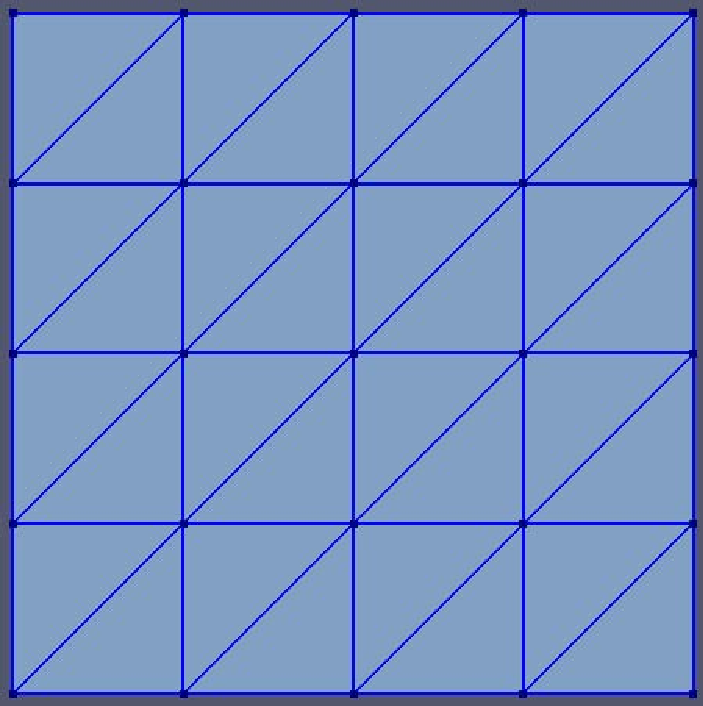
\includegraphics[width=60mm, height=60mm]{Mesh_A}
		\label{fig:subfiga}
		}
	\subfigure[Primal mesh with inner dual cells] {
		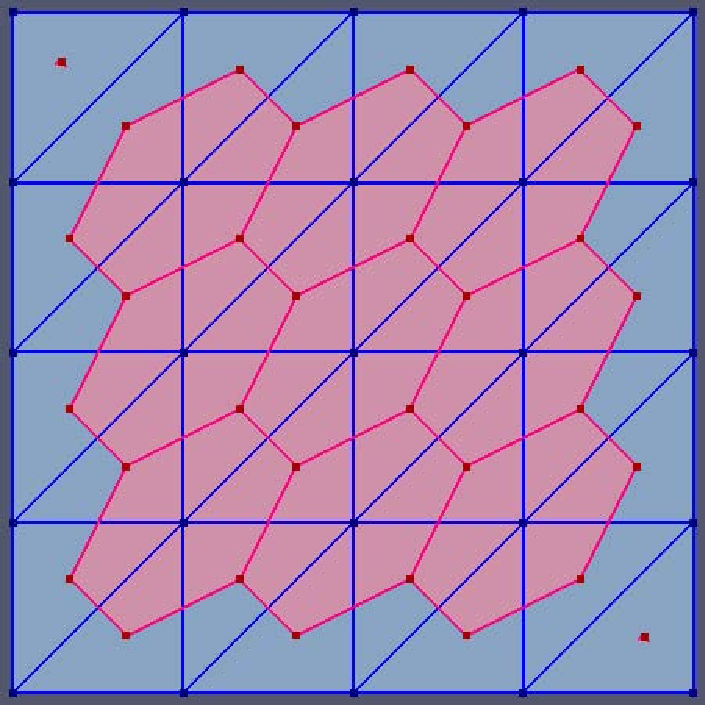
\includegraphics[width=60mm, height=60mm]{Mesh_C}
		\label{fig:subfigc}
		}
	\subfigure[Primal and dual mesh] {
		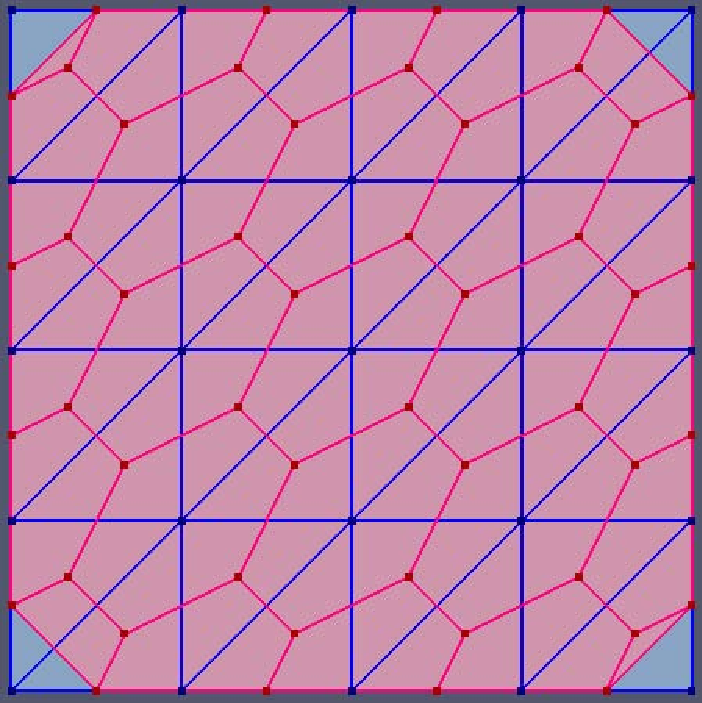
\includegraphics[width=60mm, height=60mm]{Mesh_E}
		\label{fig:subfige}
		}
	\subfigure[Dual mesh] {
		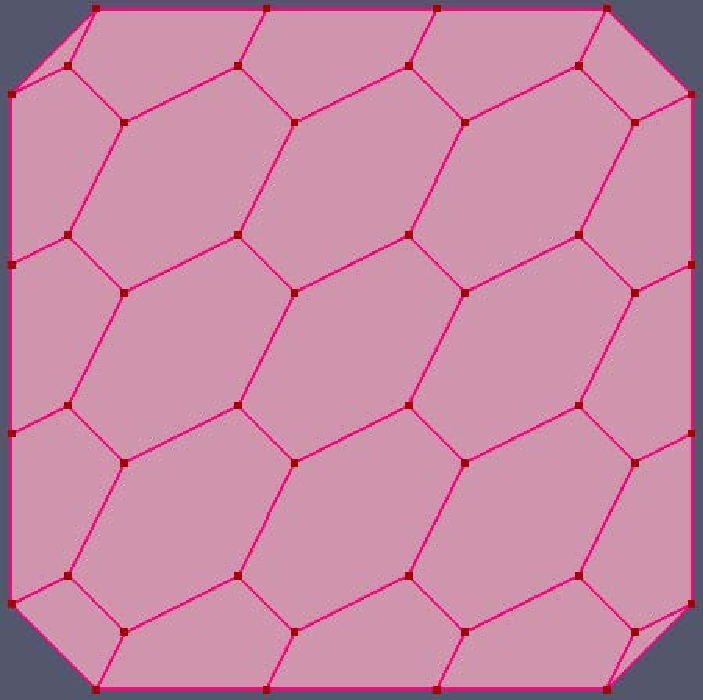
\includegraphics[width=60mm, height=60mm]{Mesh_F}
		\label{fig:subfigf}
		}
	\caption{Primal to dual mesh}
\label{fig:primal2DualMesh}
\end{figure}
For testing this data structure and filter, we deleted one primal edge and re-run the whole code for getting dual mesh. The snapshot of re-run is shown in figure~\ref{fig:primal2DualMeshwithhole}.
\begin{figure}
	\centering
	\subfigure[Primal mesh with inside hole] {
		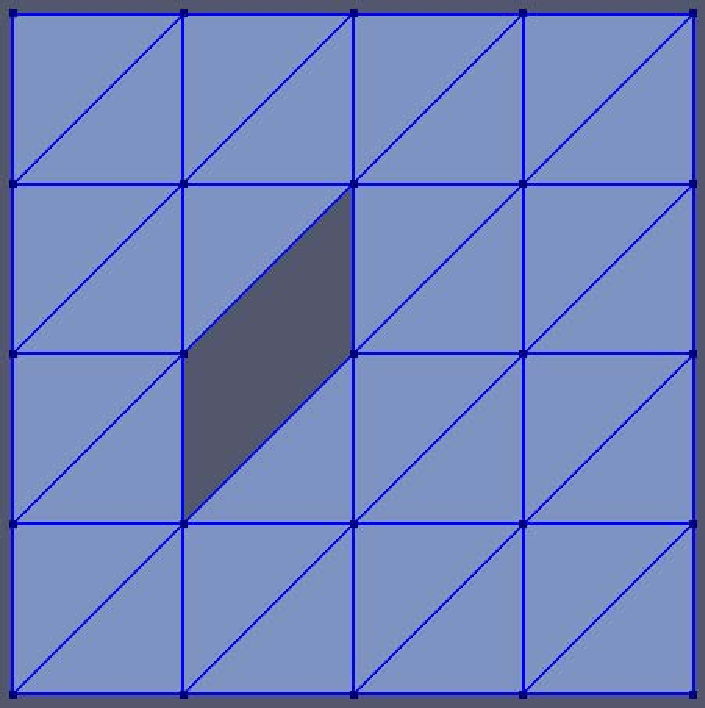
\includegraphics[width=50mm, height=50mm]{Mesh2_A}
		\label{fig:subfig2a}
		}
	\subfigure[Primal with dual mesh] {
		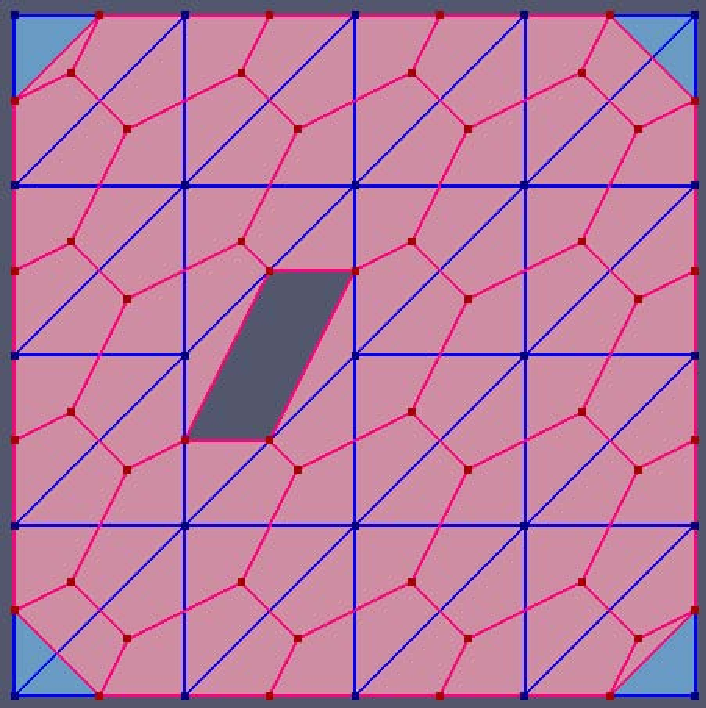
\includegraphics[width=50mm, height=50mm]{Mesh2_C}
		\label{fig:subfig2b}
		}
	\subfigure[Dual mesh with inside hole] {
		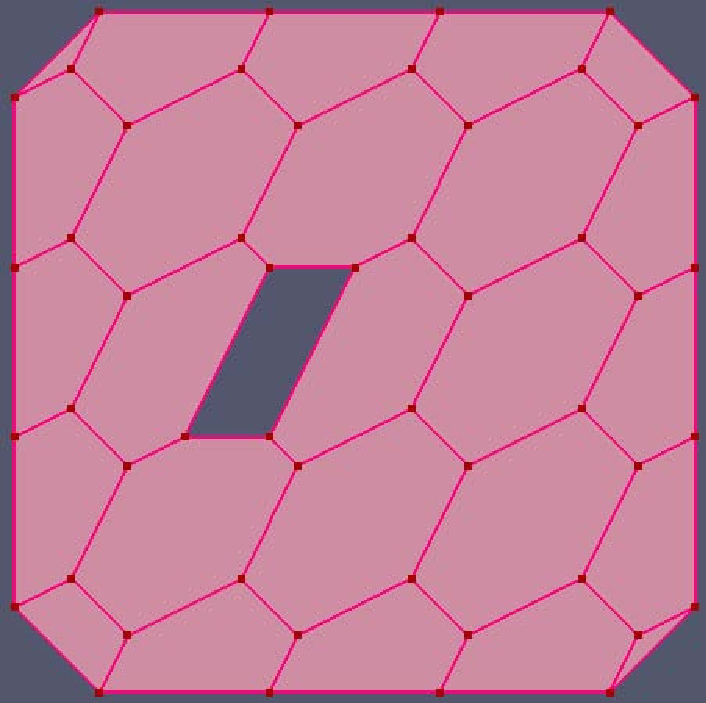
\includegraphics[width=50mm, height=50mm]{Mesh2_D}
		\label{fig:subfig2c}
		}
	\caption{Primal to dual mesh with inside hole}
\label{fig:primal2DualMeshwithhole}
\end{figure}
%-------------------------------------------------------------------------
\subsection{Test with Delaunay to Voronoi}
Using the \emph{PointSetToDelaunayTriangulationFilter} \cite{Rigaud2012b}, we tested this data structure on Delaunay mesh to Voronoi diagram. We input a planer Delaunay mesh into new data structure as shown in figure~\ref{fig:Delauny_A} and generate the corresponding Voronoi diagram by using \emph{QuadEdgeMeshToQuadEdgeMeshWithDualFilter} and the \emph{CircumcentreDualPointFunctor} as shown in figure~\ref{fig:Delauny_B}. Later, the Voronoi diagram is shown in figure~\ref{fig:Delauny_C} using new adaptor \emph{itk::QuadEdgeMeshWithDualAdaptor}.\\
\begin{figure}[!b]
	\centering
	\subfigure[Delaunay Mesh] {
		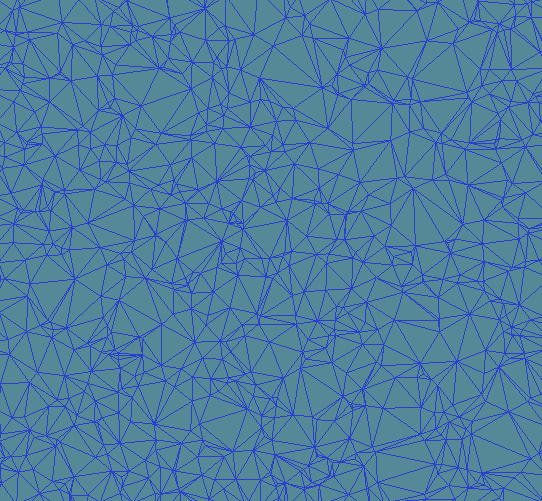
\includegraphics[width=50mm, height=50mm]{Delauny_A}
		\label{fig:Delauny_A}
		}
	\subfigure[Delaunay and Voronoi Mesh] {
		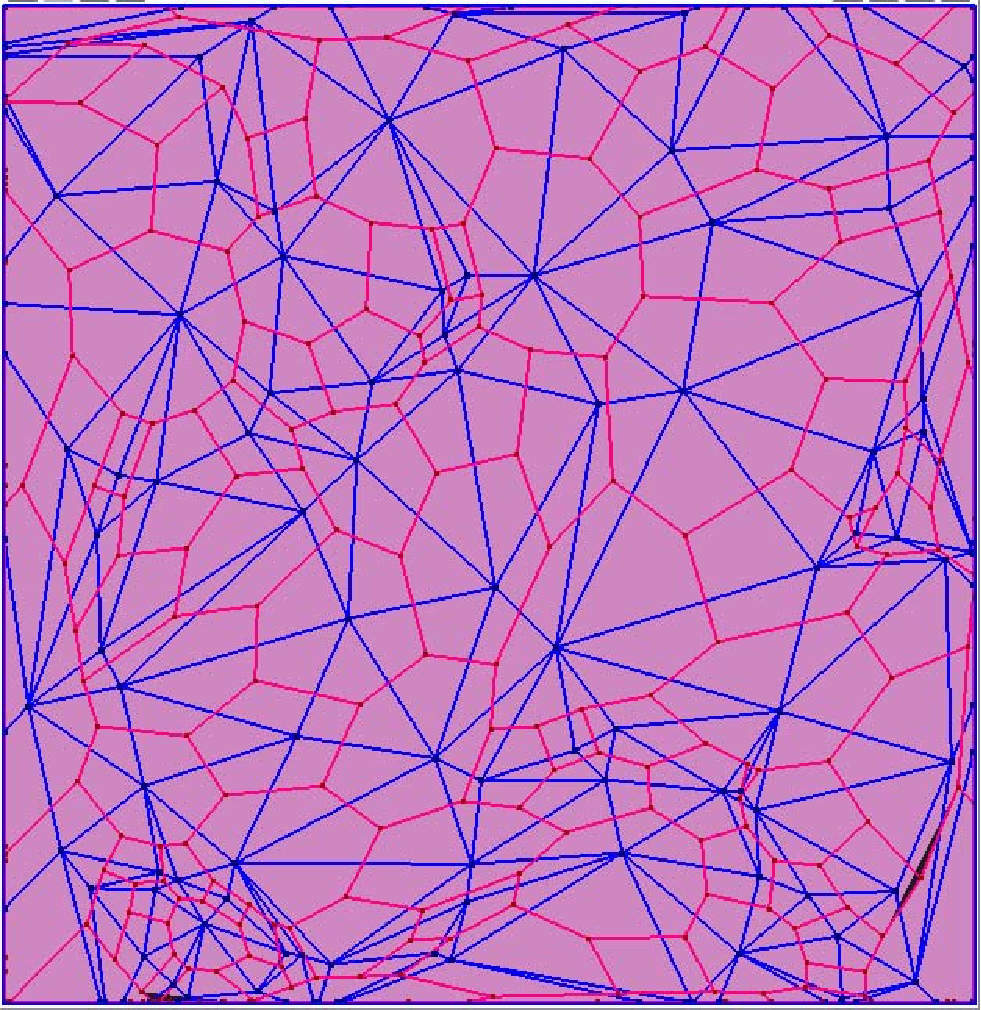
\includegraphics[width=50mm, height=50mm]{Delauny_B}
		\label{fig:Delauny_B}
		}
	\subfigure[Voronoi Mesh] {
		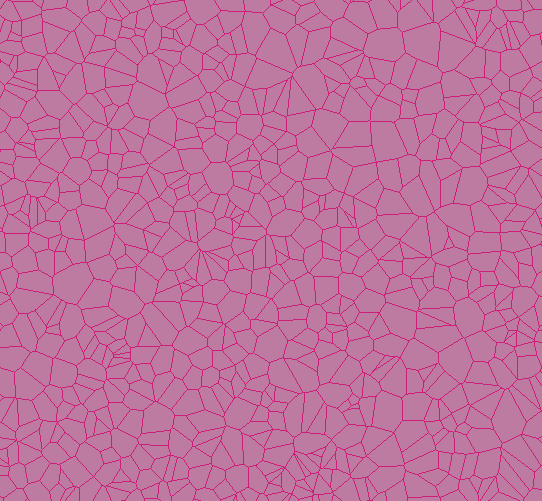
\includegraphics[width=50mm, height=50mm]{Delauny_C}
		\label{fig:Delauny_C}
		}
	\caption{Delaunay to Voronoi Mesh}
\label{fig:delaunayToVoronoiMesh}
\end{figure}
%-------------------------------------------------------------------------
\subsection{Test on non planar mesh}
We perform last test on non-planer mesh. A spherical triangulation mesh can be seen in figure~\ref{fig:Sphere_A}, generated simplex (dual) mesh along with triangulation (primal) mesh can be seen in figure~\ref{fig:Sphere_B} and finally, simplex (dual) mesh generated with new adaptor can be seen in figure~\ref{fig:Sphere_C}. \\
\begin{figure}[!b]
	\centering
	\subfigure[Non-Planer Triangulation Mesh] {
		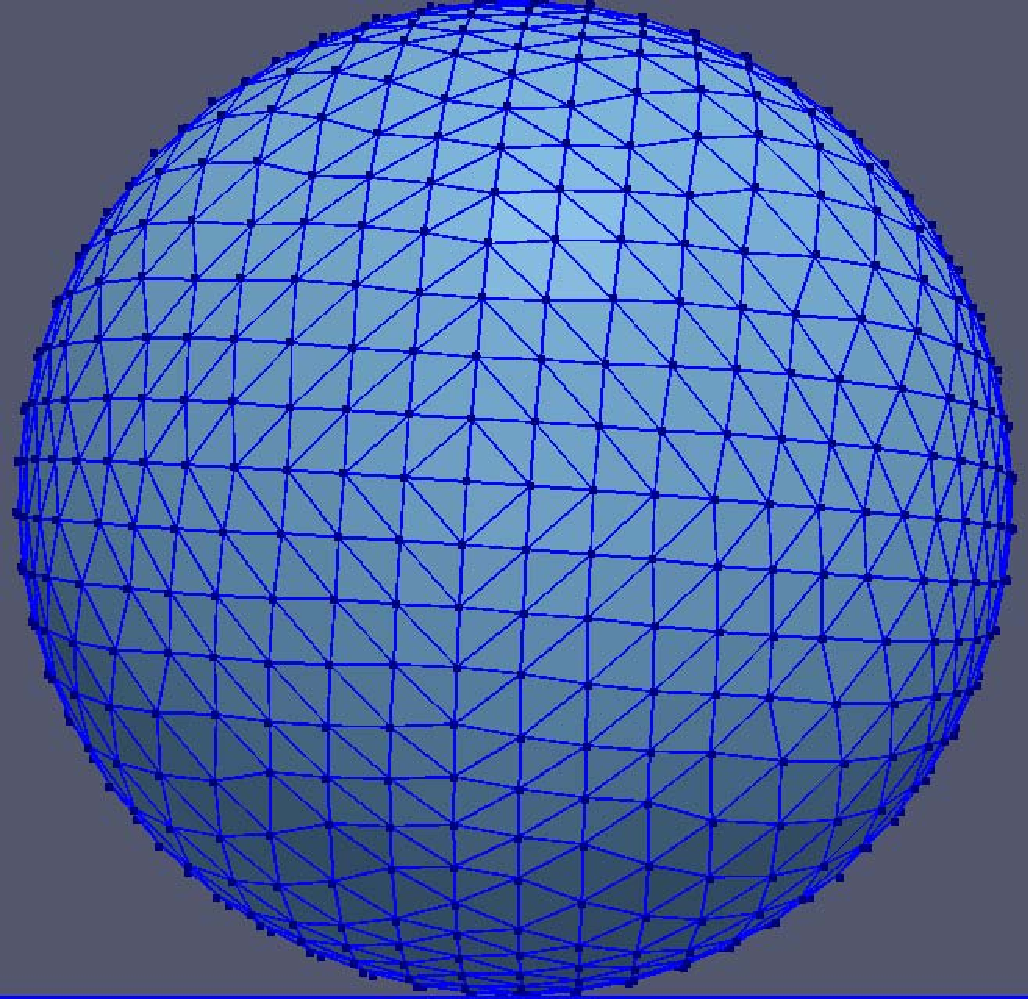
\includegraphics[width=50mm, height=50mm]{Sphere_A}
		\label{fig:Sphere_A}
		}
	\subfigure[Non-Planer Triangulation and Simplex Mesh] {
		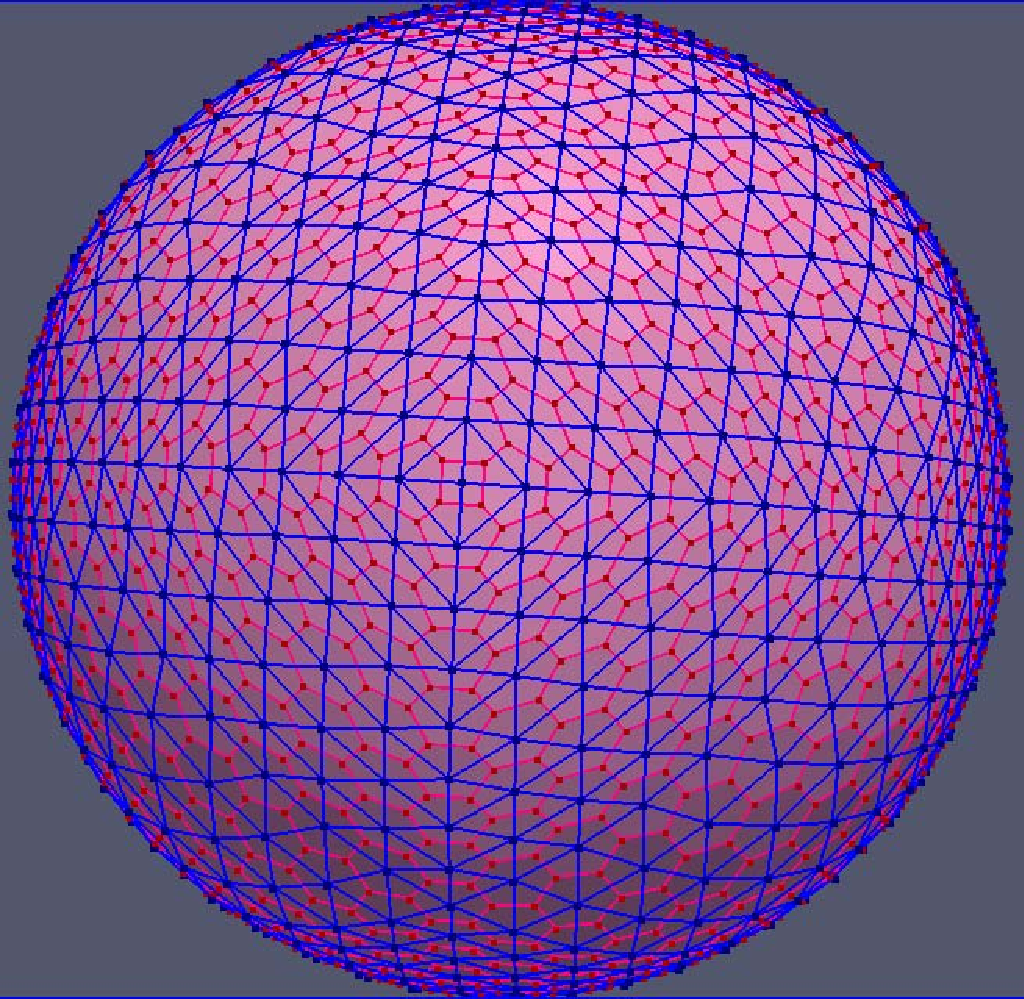
\includegraphics[width=50mm, height=50mm]{Sphere_B}
		\label{fig:Sphere_B}
		}
	\subfigure[Non-Planer Simplex Mesh] {
		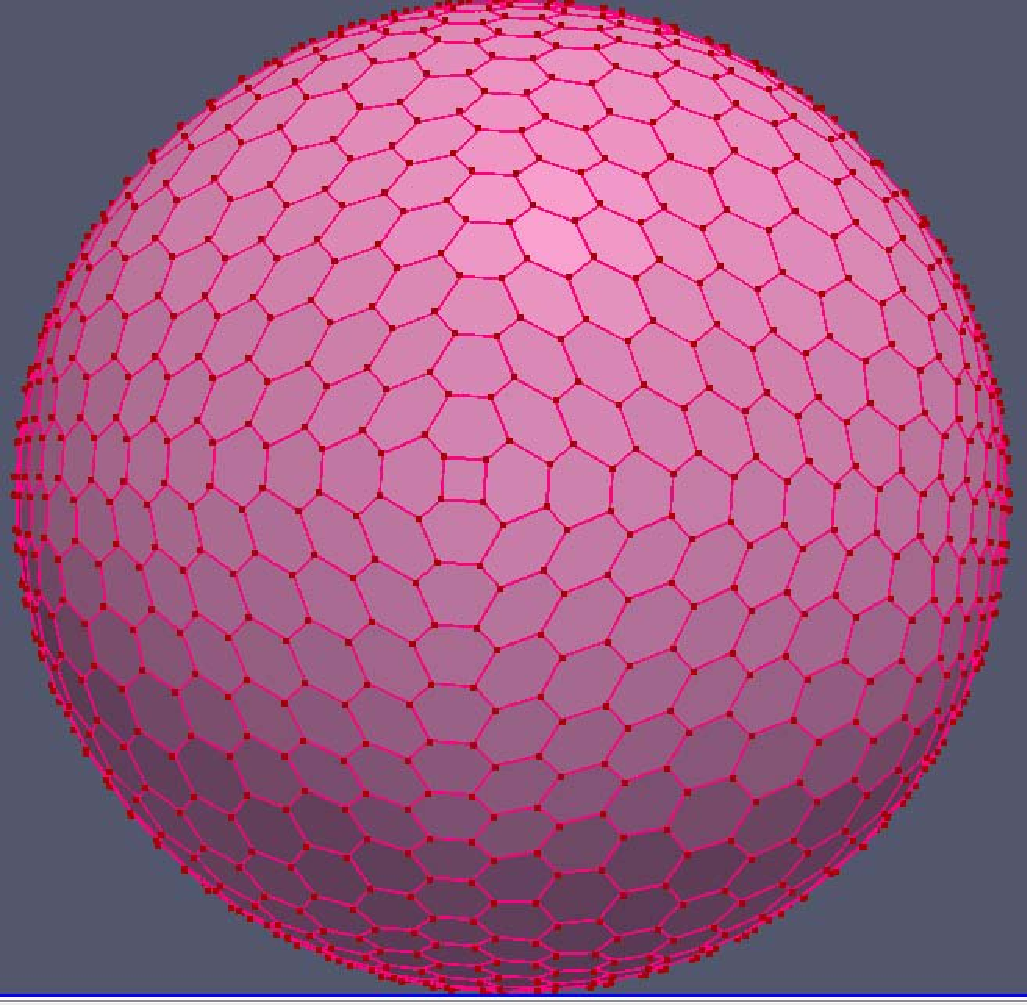
\includegraphics[width=50mm, height=50mm]{Sphere_C}
		\label{fig:Sphere_C}
		}
	\caption{Non-Planer Mesh containing (Triangulation and  Simplex Mesh)}
\label{fig:nonplanerTriangulationToSimplexMesh}
\end{figure}
%--------------------------------------------------------------------------
\section{Usage}
An example \emph{SimplexMesh.cxx} is provided with the sources and is used for the tests. The filter \emph{QuadEdgeMeshToQuadEdgeMeshWithDualFilter} is templated on float and 3 dimensions \emph{itk::QuadEdgeMeshWithDual}.
\begin{verbatim}
// Typedef definition
typedef itk::QuadEdgeMeshWithDual< float, 3 >          MeshType;
typedef itk::QuadEdgeMeshToQuadEdgeMeshWithDualFilter< MeshType >  
                                                       FillDualFilterType;
typedef itk::QuadEdgeMeshWithDualAdaptor< MeshType >   AdaptorType;

typedef itk::VTKPolyDataWriter< MeshType >    MeshWriterType;
typedef itk::VTKPolyDataWriter< AdaptorType > DualMeshWriterType;

// Create primal mesh
MeshType::Pointer myPrimalMesh = MeshType::New();
CreateSquareTriangularMesh< MeshType >( myPrimalMesh );

// Create dual mesh
FillDualFilterType::Pointer fillDual = FillDualFilterType::New();
fillDual->SetInput( myPrimalMesh );
fillDual->Update();

AdaptorType* adaptor = new AdaptorType();
adaptor->SetInput( fillDual->GetOutput() );

// Write dual mesh
DualMeshWriterType::Pointer writer = DualMeshWriterType::New();
writer->SetInput( adaptor );
writer->SetFileName( "TestSquareTriangularSimplexMesh.vtk" );
writer->Write();
\end{verbatim}


 %--- Todo -- add future work -- multiresolution, simplex eulor op, subdivision, deformable surface
\bibliographystyle{plain}
\bibliography{InsightJournal}

\end{document}

